\documentclass[tikz,border=0pt]{standalone}
% Shared TikZ style for figures in
% Layered Network Programming with SNode.C.
%
% Contract for this figure set:
% - every figure PDF has an exact 160 mm canvas width;
% - the TikZ drawing is rendered at native size, not scaled;
% - the drawing is horizontally centered on that canvas;
% - semantic colors, line widths, arrow widths, boundary titles, and spacing
%   are kept consistent unless a local exception is needed to fit the canvas.

\usepackage{xcolor}
\usepackage{tikz}
\usetikzlibrary{
  arrows.meta,
  backgrounds,
  calc,
  fit,
  matrix,
  positioning,
  shapes.geometric,
  shapes.multipart
}

% ----------------------------------------------------------------------
% Palette.
% ----------------------------------------------------------------------
\definecolor{snodecInk}{HTML}{17212B}
\definecolor{snodecMuted}{HTML}{4B5F68}
\definecolor{snodecRule}{HTML}{7A8B93}

\definecolor{snodecBlue}{HTML}{0B4F6C}
\definecolor{snodecBlueSoft}{HTML}{E3F2F8}

\definecolor{snodecGreen}{HTML}{1F7A68}
\definecolor{snodecGreenSoft}{HTML}{E5F4EF}

\definecolor{snodecOrange}{HTML}{C46A1B}
\definecolor{snodecOrangeSoft}{HTML}{FAEFE3}

\definecolor{snodecRed}{HTML}{B24A4A}
\definecolor{snodecRedSoft}{HTML}{F8E8E8}

\definecolor{snodecGraySoft}{HTML}{F1F3F2}

% Title-color palette:
% same hue family as the box, but with stronger contrast.
\colorlet{snodecTitleBlue}{snodecBlue}
\definecolor{snodecTitleGreen}{HTML}{155F51}
\definecolor{snodecTitleOrange}{HTML}{A95516}
\definecolor{snodecTitleGray}{HTML}{4B5F68}
\colorlet{snodecTitleRed}{snodecRed}

% ----------------------------------------------------------------------
% Geometry and line constants.
% ----------------------------------------------------------------------
\newcommand{\snodecCanvasHalfWidth}{80mm}
\newcommand{\snodecCanvasVMargin}{7pt}

\newcommand{\snodecBoxCorner}{2.5pt}
\newcommand{\snodecBoundaryCorner}{3pt}

\newcommand{\snodecBoxLineWidth}{0.70pt}
\newcommand{\snodecInnerLineWidth}{0.58pt}
\newcommand{\snodecBoundaryLineWidth}{0.58pt}
\newcommand{\snodecArrowLineWidth}{0.70pt}
\newcommand{\snodecSecondaryLineWidth}{0.58pt}
\newcommand{\snodecBusLineWidth}{0.58pt}

\newcommand{\snodecBoxXSep}{3mm}
\newcommand{\snodecBoxYSep}{2.5mm}
\newcommand{\snodecSmallBoxXSep}{1.2mm}
\newcommand{\snodecSmallBoxYSep}{1.6mm}
\newcommand{\snodecBoundaryInnerSep}{4.5mm}

\newcommand{\snodecGapSmall}{6mm}
\newcommand{\snodecGapNormal}{8mm}
\newcommand{\snodecGapLarge}{11mm}
\newcommand{\snodecGapMajor}{14mm}
\newcommand{\snodecBendLeg}{6mm}
\newcommand{\snodecOutsideLane}{8mm}

% ----------------------------------------------------------------------
% Shared TikZ styles.
% ----------------------------------------------------------------------
\tikzset{
  snodec diagram/.style={
    font=\sffamily\small,
    text=snodecInk,
    line cap=round,
    line join=round,
    >=Latex
  },
  snodec base box/.style={
    rounded corners=\snodecBoxCorner,
    line width=\snodecBoxLineWidth,
    align=center,
    inner xsep=\snodecBoxXSep,
    inner ysep=\snodecBoxYSep
  },
  snodec runtime box/.style={
    snodec base box,
    draw=snodecBlue!78,
    fill=snodecBlueSoft
  },
  snodec application box/.style={
    snodec base box,
    draw=snodecGreen!78,
    fill=snodecGreenSoft
  },
  snodec protocol box/.style={
    snodec base box,
    draw=snodecOrange!80,
    fill=snodecOrangeSoft
  },
  snodec neutral box/.style={
    snodec base box,
    draw=snodecRule!85,
    fill=snodecGraySoft
  },
  snodec failure box/.style={
    snodec base box,
    draw=snodecRed!82,
    fill=snodecRedSoft
  },
  snodec inner box/.style={
    snodec neutral box,
    line width=\snodecInnerLineWidth,
    inner xsep=\snodecSmallBoxXSep,
    inner ysep=\snodecSmallBoxYSep
  },
  snodec boundary/.style={
    draw=snodecRule!82,
    dashed,
    rounded corners=\snodecBoundaryCorner,
    line width=\snodecBoundaryLineWidth,
    inner sep=\snodecBoundaryInnerSep
  },
  snodec boundary title/.style={
    font=\sffamily\bfseries\small,
    text=snodecTitleBlue,
    fill=white,
    fill opacity=1,
    text opacity=1,
    draw=none,
    anchor=center,
    text height=1.6ex,
    text depth=.25ex,
    inner xsep=1.6pt,
    inner ysep=0.8pt
  },
  snodec arrow label/.style={
    font=\sffamily\bfseries\footnotesize,
    text=snodecInk,
    fill=white,
    fill opacity=1,
    text opacity=1,
    draw=none,
    inner sep=1.0pt
  },
  snodec main arrow/.style={
    -{Latex[length=2.2mm,width=1.6mm]},
    line width=\snodecArrowLineWidth,
    draw=snodecMuted!76
  },
  snodec secondary arrow/.style={
    -{Latex[length=2.0mm,width=1.4mm]},
    line width=\snodecSecondaryLineWidth,
    draw=snodecMuted!68
  },
  snodec bus line/.style={
    draw=snodecMuted!72,
    line width=\snodecBusLineWidth
  },
  snodec return arrow/.style={
    snodec secondary arrow,
    dashed,
    draw=snodecMuted!72
  },
  snodec note/.style={
    font=\sffamily\footnotesize,
    text=snodecMuted,
    align=center
  },
  snodec label/.style={
    font=\sffamily\bfseries\small,
    text=snodecTitleBlue
  },
  % Backward-compatible aliases for old figure sources.
  snodec box/.style={snodec runtime box},
  snodec layer/.style={snodec runtime box,text width=48mm,minimum height=9mm},
  snodec role/.style={snodec application box,text width=38mm},
  snodec protocol/.style={snodec protocol box,text width=42mm},
  snodec neutral/.style={snodec neutral box,text width=42mm},
  snodec failure/.style={snodec failure box,text width=42mm},
  snodec arrow/.style={snodec main arrow,draw=snodecBlue!70},
  snodec muted arrow/.style={snodec secondary arrow}
}

% Fixed-width page/canvas helper. The drawing is not scaled. The natural
% drawing is centered horizontally on a 160 mm wide canvas.
\newcommand{\snodecApplyFixedCanvas}{%
  \coordinate (snodecCanvasCenter) at (current bounding box.center);%
  \coordinate (snodecCanvasSW)%
    at ($(snodecCanvasCenter)+(-\snodecCanvasHalfWidth,0)$ |- current bounding box.south);%
  \coordinate (snodecCanvasNE)%
    at ($(snodecCanvasCenter)+(\snodecCanvasHalfWidth,0)$ |- current bounding box.north);%
  \path[use as bounding box]
    ([yshift=-\snodecCanvasVMargin]snodecCanvasSW)
    rectangle
    ([yshift=\snodecCanvasVMargin]snodecCanvasNE);%
}


\begin{document}
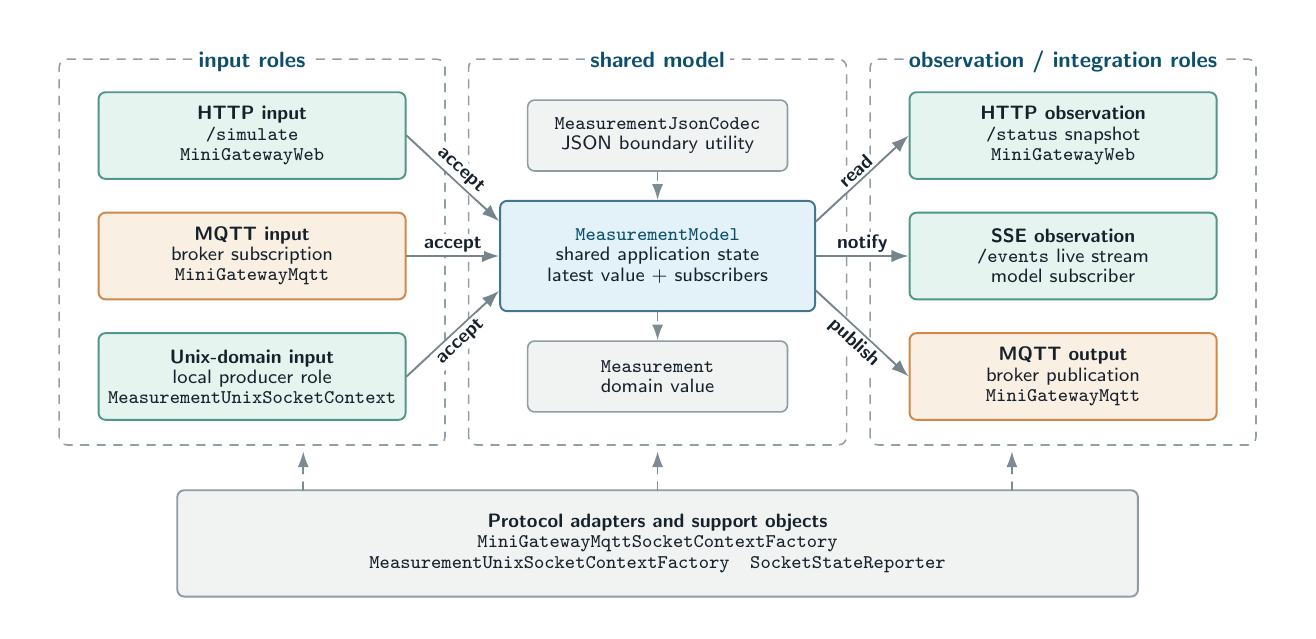
\begin{tikzpicture}[
  x=1mm,y=1mm,
  snodec diagram,
  every node/.style={text=snodecInk, align=center},
  group label/.style={snodec boundary title, font=\sffamily\bfseries\footnotesize, text=snodecTitleBlue, inner xsep=1.8pt, inner ysep=0.8pt},
  role/.style={snodec application box, rounded corners=\snodecBoxCorner, line width=\snodecBoxLineWidth, minimum width=39mm, minimum height=11mm, inner xsep=1.0mm, inner ysep=0.9mm, font=\sffamily\scriptsize},
  mqtt/.style={snodec protocol box, rounded corners=\snodecBoxCorner, line width=\snodecBoxLineWidth, minimum width=39mm, minimum height=11mm, inner xsep=1.0mm, inner ysep=0.9mm, font=\sffamily\scriptsize},
  model/.style={snodec runtime box, rounded corners=\snodecBoxCorner, line width=\snodecBoxLineWidth, minimum width=40mm, minimum height=14mm, inner xsep=1.2mm, inner ysep=1.2mm, font=\sffamily\scriptsize},
  util/.style={snodec inner box, rounded corners=\snodecBoxCorner, line width=\snodecInnerLineWidth, minimum width=33mm, minimum height=9mm, inner xsep=0.9mm, inner ysep=0.8mm, font=\sffamily\scriptsize},
  support/.style={snodec neutral box, rounded corners=\snodecBoxCorner, line width=\snodecBoxLineWidth, minimum width=122mm, minimum height=13.5mm, inner xsep=1.2mm, inner ysep=1.0mm, font=\sffamily\scriptsize},
  flow/.style={snodec main arrow},
  supportflow/.style={snodec return arrow}
]

% Fixed 160 mm canvas.
\path[use as bounding box] (-80,-45) rectangle (80,29);

% Group boundaries use the shared dashed boundary style.
\draw[snodec boundary] (-76,-24) rectangle (-27,25);
\node[group label] at (-51.5,25) {input roles};

\draw[snodec boundary] (-24,-24) rectangle (24,25);
\node[group label] at (0,25) {shared model};

\draw[snodec boundary] (27,-24) rectangle (76,25);
\node[group label] at (51.5,25) {observation / integration roles};

% Center model group.
\node[util] (codec) at (0,15.3) {\texttt{MeasurementJsonCodec}\\[-0.2mm]JSON boundary utility};
\node[model] (model) at (0,0) {\textbf{\textcolor{snodecTitleBlue}{\texttt{MeasurementModel}}}\\[-0.3mm]shared application state\\[-0.2mm]latest value + subscribers};
\node[util] (value) at (0,-15.3) {\texttt{Measurement}\\[-0.2mm]domain value};

% Input roles.
\node[role] (httpSim) at (-51.5,15.3) {\textbf{HTTP input}\\[-0.25mm]\texttt{/simulate}\\[-0.25mm]\texttt{MiniGatewayWeb}};
\node[mqtt] (mqttIn) at (-51.5,0) {\textbf{MQTT input}\\[-0.25mm]broker subscription\\[-0.25mm]\texttt{MiniGatewayMqtt}};
\node[role] (unixIn) at (-51.5,-15.3) {\textbf{Unix-domain input}\\[-0.25mm]local producer role\\[-0.25mm]\texttt{MeasurementUnixSocketContext}};

% Observation and integration roles.
\node[role] (httpStatus) at (51.5,15.3) {\textbf{HTTP observation}\\[-0.25mm]\texttt{/status} snapshot\\[-0.25mm]\texttt{MiniGatewayWeb}};
\node[role] (sseEvents) at (51.5,0) {\textbf{SSE observation}\\[-0.25mm]\texttt{/events} live stream\\[-0.25mm]model subscriber};
\node[mqtt] (mqttOut) at (51.5,-15.3) {\textbf{MQTT output}\\[-0.25mm]broker publication\\[-0.25mm]\texttt{MiniGatewayMqtt}};

% Bottom support band, kept close enough to the role groups while leaving visible separation.
\node[support] (support) at (0,-36.5) {\textbf{Protocol adapters and support objects}\\[-0.25mm]\texttt{MiniGatewayMqttSocketContextFactory}\\[-0.25mm]\texttt{MeasurementUnixSocketContextFactory}\quad\texttt{SocketStateReporter}};

% Distributed model-border anchor points.
\coordinate (modelLWTop) at ($(model.west)+(0,4.4mm)$);
\coordinate (modelLWMid) at (model.west);
\coordinate (modelLWBot) at ($(model.west)+(0,-4.4mm)$);
\coordinate (modelRETop) at ($(model.east)+(0,4.4mm)$);
\coordinate (modelREMid) at (model.east);
\coordinate (modelREBot) at ($(model.east)+(0,-4.4mm)$);

% Main data/control flow arrows.
\draw[flow] (httpSim.east) -- node[snodec arrow label, font=\sffamily\bfseries\scriptsize, sloped, above] {accept} (modelLWTop);
\draw[flow] (mqttIn.east) -- node[snodec arrow label, font=\sffamily\bfseries\scriptsize, above] {accept} (modelLWMid);
\draw[flow] (unixIn.east) -- node[snodec arrow label, font=\sffamily\bfseries\scriptsize, sloped, below] {accept} (modelLWBot);

\draw[flow] (modelRETop) -- node[snodec arrow label, font=\sffamily\bfseries\scriptsize, sloped, above] {read} (httpStatus.west);
\draw[flow] (modelREMid) -- node[snodec arrow label, font=\sffamily\bfseries\scriptsize, above] {notify} (sseEvents.west);
\draw[flow] (modelREBot) -- node[snodec arrow label, font=\sffamily\bfseries\scriptsize, sloped, below] {publish} (mqttOut.west);

% Utility support inside the shared model group.
\draw[supportflow] (codec.south) -- (model.north);
\draw[supportflow] (model.south) -- (value.north);

% Support arrows from the adapter/support band. They stop outside the dashed role groups.
\draw[supportflow] (-45,-29.75) -- (-45,-24.8);
\draw[supportflow] (0,-29.75) -- (0,-24.8);
\draw[supportflow] (45,-29.75) -- (45,-24.8);

\end{tikzpicture}
\end{document}
